\documentclass[twocolumn]{article}
\usepackage{graphicx}
\usepackage{tikz}
\usepackage{float}
\usepackage{listings}
\usepackage{amsmath}
\usepackage[utf8]{inputenc}
\usepackage{hyperref} % For hyperlinks

\usetikzlibrary{shapes.geometric, arrows.meta, positioning, matrix, 3d, calc}

\usepackage{color}
\definecolor{darkblue}{rgb}{0.0, 0.0, 0.3}
\hypersetup{
    colorlinks=true,
    linkcolor=darkblue,
    filecolor=darkblue,      
    urlcolor=darkblue,
    citecolor=darkblue,
}


\title{Take Me One More: Efficient Clustering Compression using Inter-Frame Encoding}
\author{Ignacio Brasca}
\date{\today}
\setlength{\parskip}{1em}
\begin{document}

\maketitle

\begin{abstract}
    \textit{This paper introduces a novel data encoding compression algorithm aimed at significantly reducing storage requirements for quick-capture devices, such as CCTV cameras and smartphones. By leveraging Huffman coding alongside Discrete Cosine Transform (DCT) techniques, the proposed algorithm offers an efficient solution for minimizing data file sizes. Unlike traditional image compression methods that treat each frame independently, our approach utilizes inter-frame encoding to exploit temporal redundancies between consecutive frames, achieving higher compression ratios while maintaining image quality. The algorithm's workflow, implementation details, and its application in dynamic cluster formation and memory optimization are discussed, alongside case studies demonstrating its effectiveness in various real-world scenarios.}
    \end{abstract}
    
    \textbf{Keywords:} \textit{intraframe data encoding, compression algorithm, Huffman coding, Discrete Cosine Transform (DCT), inter-frame encoding, dynamic cluster formation, memory optimization, data compression}    
    

\section{Introduction}
In recent times, there has been a surge in the need for efficient data compression techniques due to the rapid expansion of quick-capture devices like CCTV cameras, smartphones, and other portable storage-constrained devices. In response to this challenge, there's formulated in this essay a potential concept for an intraframe data encoding compression algorithm that allows reduction of storage requirements. This proposed algorithm leverages the power of Huffman coding and Discrete Cosine Transform (DCT) techniques, which are highly effective in minimizing the size of data files.

Using Huffman coding as a form of entropy encoding technique that replaces a sequence of symbols with shorter codes based on their probability distribution we can save storage in benefit of redundancy \cite{van1976construction}. In contrast, DCT is a mathematical process \cite{narasimha1978computation} that decomposes an image into a series of frequency components and helps reduce the redundancy as well, in pictures as well as video frames (pictures in a time-series). Combining these two powerful techniques, the proposed algorithm can offer significant storage savings for quick-capture devices.

The method here proposed allow us to understand not only one picture as a whole but an ecosystem of similar pictures \cite{lee2002compressing} based on a timestamp technique. Enabling us the categorization based a on threshold generated after a difference threshold computed using the inception frame. This technique has been in used in the past for video compression \cite{wang2012memory}, but not for single images. This essay will provide an overview of the inter-frame encoding algorithm, its workflow, implementation details, and case studies to demonstrate its effectiveness.

\section{Background}
Traditional image compression techniques, such as JPEG and PNG, rely on compressing individual frames independently. While these methods are effective for compressing individual images, they may not be optimal for sequences of similar images when those are being captured by real-time devices or smart phones. inter-frame encoding help us to overpass this limitation by exploiting the temporal redundancy between consecutive frames in a sequence. By storing only the differences between frames, inter-frame encoding can achieve higher compression ratios while preserving image quality.

\subsection{Formal Definitions}

\begin{enumerate}
    \item \textbf{Inception Frame $(I)$:} The first frame in a sequence of images.
    \item \textbf{Beam $(beam_{n,m})$:} A data point in a frame that can be modified using a set of operations.
    \item \textbf{Difference Threshold $(N)$:} The maximum difference allowed between consecutive frames to be considered similar.
    \item \textbf{Cluster Frames $(K)$:} A group of similar images within the difference threshold.
\end{enumerate}


\subsection{Sequence Compression Against a Set of Frames}
To introduce the underlying techniques, we can define a set of frames $K$ as a set of frames that are part of a sequence of images. Ideally, a set of images computed with this technique will use a limitation of $N$ frames, where $N$ is the amount of frames we want to compute the difference against in a timeframe $t$.

For a set of frames as
$$
K = \{X_1,X_2,X_3\}
$$
As soon as we cluster them down, we can define a set of expressions we can perform at the frame level as  $$X_{k} = X_{n} \circ X_{m}$$ whereas we can also combine these to produce a new $X_{k}$ frame based on the statement generated after the application of expressions.

Operations $\circ$ can be computed at runtime, where a new piece of information appears in the set of $K$ frames, and this will be included in the set of new data points $K$. 

A data point part of $K$ will be called a $beam$ and will be part of a set of $beams_{n,m}$ where $n,m$ are the dimensions restrictions of the matrix containing all the beams available in the source of information presented as a frame in $K$.

\subsection{Restrictions}
There are a few restrictions we need to take into account when computing the difference between frames in a sequence of images:

\begin{enumerate}
    \item We need to compute always the same amount of information in a finite combination of RGB values; this means each frame should contain at least $\max(X_n)$ pixels, where $X_n$ is the frame with the highest amount of color depth (information per pixel).
    \item ${len}(K)$ should always be higher than 1 where $K$ is the set of frames we want to compute the difference against.
    \item $X_{n} \circ X_{m}$ should always output a valid matrix as a result.
\end{enumerate}

Operations available at the $beam$ level are placed uttermost in the front of any pixel transformation technique available, always using the inter-frame perspective of the information account.

In case multiple beams $x_{i,j}$ would be intertwined, we can define a net set of operations to establish what or which part of the frames we want to modify during which amount of time.

\subsection{Inception frame}
Currently, compression against a set of frames is being computed against a linear relationship where $K$ frames are only compressed after $N$ times during a $t$ span. Presented here is the utilization of a global difference matrix called $K_{global}$ where we track against a set of values used on the same matrix as it was a memory registry.

Starting from frame $n$, we can compute and utilize the same amount of $beams_{n,m}$ already stored from the initial inception frame. 

From an $inception$ frame, we should always compute the difference against the same amount of frames, where $n$ is the frame we want to compute the difference against and then evaluate if the difference threshold is small enough to be considered part of the same cluster.

Operations $\circ$ can be computed at runtime, against a set of $beams_{n,m}$ where $n,m$ are the dimensions restrictions of the matrix containing all the beams available in the source of information presented as a frame in $K$. This information is beneficial in order to calculate not only the difference between frames but also to compute inception frame to obtain the same set of frames in a different time span $t$.

\subsection{Reverting frames}
In order to revert an operation $\circ$, we can simply apply the inverse operation $\circ^{-1}$ to the frame $X_{k}$ and obtain the original frame $X_{n}$ or $X_{m}$. This operation is only possible if the original frame $X_{n}$ or $X_{m}$ is available in the set of frames $K$.

\section{Architecture}
The proposed two-step architecture for processing frames in a cluster of pictures is designed to efficiently analyze a series of images while minimizing redundancy and memory usage. The first part involves dynamically defining image clusters, where each cluster consists of images with similar content up to a specified threshold. Images exceeding the threshold are considered distinct and initiate a new cluster. The second part focuses on optimizing memory and efficiently matching differences between frames to avoid processing redundant information.

The two steps in the proposed architecture can be named as follows:

\begin{enumerate}
    \item Dynamic Cluster Formation (DCF)
    \item Memory Optimization and Inter-frame Matching (MOIM)
\end{enumerate}

\subsection{Dynamic Cluster Formation}
The technique here described (Dynamic Cluster Formation) or from now on: DCF, is an step that continuously checks for changes in the input stream of images based on a initial timestamp. When a difference greater than a defined threshold is detected, the current cluster is considered complete, and a new cluster begins. This step ensures that similar images are grouped together, allowing for efficient inter-frame encoding.

\begin{figure}[!h]
    \centering
    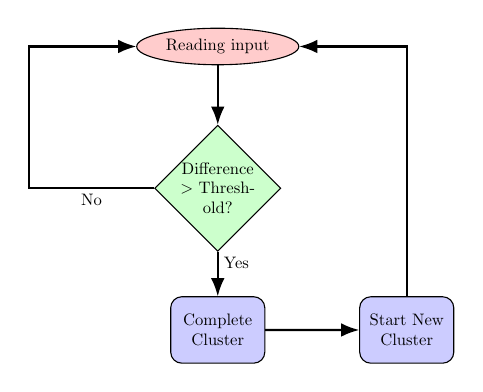
\begin{tikzpicture}[
        scale=0.80, every node/.style={scale=0.75, transform shape},
        node distance=2cm, auto, >=Latex,
        decision/.style={diamond, draw, fill=green!20, text width=4.5em, text badly centered, node distance=3cm, inner sep=0pt},
        block/.style={rectangle, draw, fill=blue!20, text width=5em, text centered, rounded corners, minimum height=4em},
        line/.style={draw, thick, -Latex},
        check/.style={draw, ellipse,fill=red!20, node distance=3cm, align=center},
    ]

    % Nodes
    \node [check] (input) {Reading input};
    \node [decision, below of=input] (decision) {Difference \\ $>$ Threshold?};
    \node [block, below of=decision, node distance=3cm] (complete) {Complete Cluster};
    \node [block, right of=complete, node distance=4cm] (new) {Start New Cluster};
    
    % Arrows
    \path [line] (input) -- (decision);
    \path [line] (decision) -- node [near start] {Yes} (complete);
    \path [line] (decision) -| node [near start] {No} ++(-3,0) |- (input);
    \path [line] (complete) -- (new);
    \path [line] (new) |- (input);

    \end{tikzpicture}
    \caption{Dynamic Cluster Formation (DCF) Step Diagram}
    \label{fig:figure1}
\end{figure}

The DCF step can be implemented using a variety of techniques, such as threshold-based clustering, k-means clustering, or hierarchical clustering. The choice of clustering technique depends on the specific requirements of the application and the nature of the input data. For images, we recommend the usage of a threshold-based clustering technique, where the difference between consecutive frames is compared against a user-defined threshold during a timeframe $t$.

The DCF step is essential for efficiently grouping similar images into clusters, which can then be processed using the technique described in the next section.

\subsection{Memory Optimization and Inter-frame Matching}
The $MOIM$ step aims to minimize redundant processing and memory usage. It matches differences between frames and avoids reprocessing frames with similar information. This optimization step is crucial for achieving high compression ratios and efficient processing. (View Figure \ref{fig:figure2})

Proposed here is the utilization of a global difference matrix called $K_{global}$, where we track against a set of values used on the same matrix as if it were a memory registry. This matrix will be used to compute the difference between frames and then evaluate if the difference threshold is small enough to be considered part of the same cluster.

Huffman coding and Discrete Cosine Transform (DCT) techniques can be applied to the differences between frames to achieve high compression ratios. This step also involves managing memory efficiently to minimize the computational overhead of processing differences (see Annex \ref{appendix:a} for more information). In collaboration with the first step of this pipeline, $MOIM$ ensures that the encoding algorithm can achieve high compression ratios while maintaining image quality.

\begin{figure}[!hb]
    \centering
    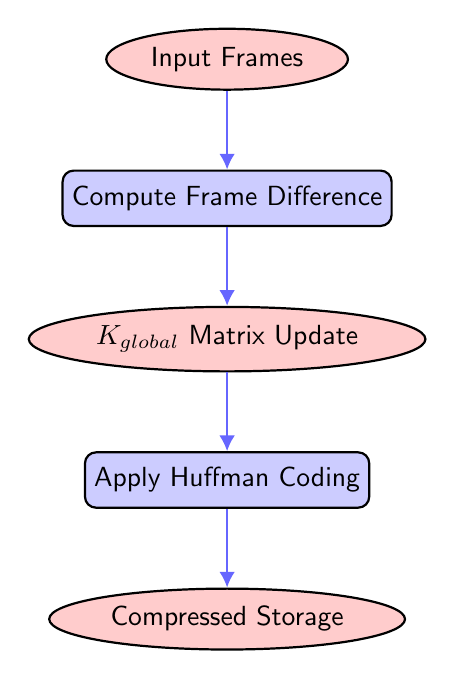
\begin{tikzpicture}[
        font=\sffamily,
        >={Latex[width=2mm,length=2mm]},
        base/.style={draw, thick, align=center, minimum height=2em, minimum width=3em, fill=blue!20},
        process/.style={base, rectangle, rounded corners},
        data/.style={base, ellipse, fill=red!20},
        arrow/.style={->, thick, color=blue!60}
    ]

    % Nodes
    \node[data] (input) {Input Frames};
    \node[process, below=of input] (compute) {Compute Frame Difference};
    \node[data, below=of compute] (globalDiff) {$K_{global}$ Matrix Update};
    \node[process, below=of globalDiff] (applyCoding) {Apply Huffman Coding};
    \node[data, below=of applyCoding] (storage) {Compressed Storage};

    % Arrows
    \draw[arrow] (input) -- (compute);
    \draw[arrow] (compute) -- (globalDiff);
    \draw[arrow] (globalDiff) -- (applyCoding);
    \draw[arrow] (applyCoding) -- (storage);

    \end{tikzpicture}
    \caption{Memory Optimization and Inter-frame Matching (MOIM) Step Diagram}
    \label{fig:figure2}
\end{figure}

\section{Clustering Encoding}
Applying the inter-frame encoding algorithm works by computing the difference between consecutive frames inside a cluster in a time sequence $t$. Let $K_{t}$ represent the $t$-th frame in the sequence, and $K_{t-1}$ represent the previous frame. The difference between $K_{t}$ and $K_{t-1}$ is computed as follows:
\[
\Delta K_{t} = K_{t} - K_{t-1}
\]
The difference $\Delta K_{t}$ is then stored using techinques expressed in the previous section along with any additional information required for reconstruction.

The inter-frame encoding algorithm can be applied to a wide range of applications, including video compression \cite{belyaev2023efficient} \cite{girod2005distributed} \cite{koga1981statistical}, medical imaging, and remote sensing. By exploiting temporal redundancy between consecutive frames, inter-frame encoding can achieve high compression ratios while maintaining image quality. As you can see in Figure \ref{fig:figure3} this process is repeated for the entire sequence of $K$ frames.

\begin{figure}[!hb]
    \centering
    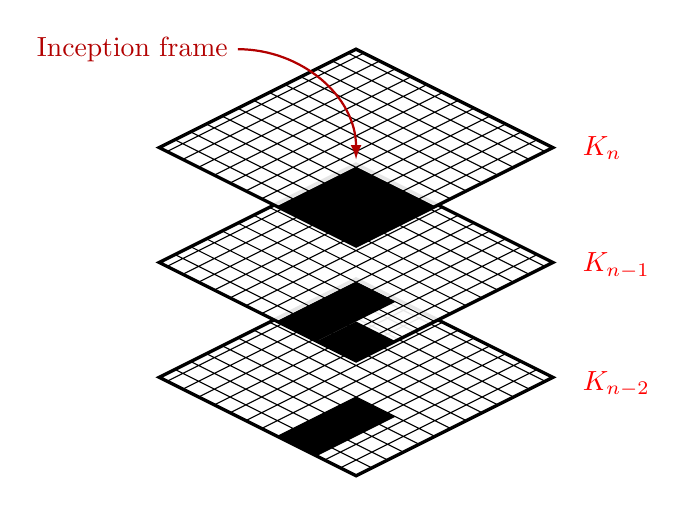
\begin{tikzpicture}[scale=.5,every node/.style={minimum size=0.5cm},on grid]
        % Bottom layer (Layer 1)
        \begin{scope}[
            yshift=-166,every node/.append style={
            yslant=0.5,xslant=-1},yslant=0.5,xslant=-1
            ]
            \draw[step=4mm, black] (0,0) grid (5,5);
            \draw[black,very thick] (0,0) rectangle (5,5);
            \fill[black] (0,1) rectangle (2,2); % bottom-left
        \end{scope}
        
        % Middle layer (Layer 2)
        \begin{scope}[
            yshift=-83,every node/.append style={
            yslant=0.5,xslant=-1},yslant=0.5,xslant=-1
            ]
            \fill[white,fill opacity=0.9] (0,0) rectangle (5,5);
            \draw[step=4mm, black] (0,0) grid (5,5);
            \draw[black,very thick] (0,0) rectangle (5,5);
            \fill[black] (0,0) rectangle (1,1); % bottom-left
            \fill[black] (0,1) rectangle (2,2); % bottom-left
        \end{scope}

        % Top layer (Layer 3)
        \begin{scope}[
            yshift=0,every node/.append style={
            yslant=0.5,xslant=-1},yslant=0.5,xslant=-1
            ]
            \fill[white,fill opacity=0.9] (0,0) rectangle (5,5);
            \draw[black,very thick] (0,0) rectangle (5,5);
            \draw[step=4mm, black] (0,0) grid (5,5);
            \fill[black] (0,0) rectangle (2,2); % bottom-left
        \end{scope}

        % Labeling
        \draw[-latex,thick,red!70!black](-3,5)node[left]{Inception frame}
            to[out=0,in=90] (0,2.2);

        \draw[thick,red](5.5,2.5)node[right]{$K_{n}$};
        \draw[thick,red](5.5,-0.5)node[right]{$K_{n-1}$};
        \draw[thick,red](5.5,-3.5)node[right]{$K_{n-2}$};

    \end{tikzpicture}
    \caption{Inter-frame Encoding Diagram}
    \label{fig:figure3}
\end{figure}

\section{Performance Metrics}
Performance rely on the reduction of redundancy and the minimization of memory usage. The following metrics can be used to evaluate the performance of the encoding algorithm:

\begin{enumerate}
    \item Compression Ratio: The ratio of the original file size to the compressed file size.
    \item Memory Usage: The amount of memory required to store the compressed metadata and reconstructed frames.
    \item Processing Time: The time required to encode and decode the differences.
    \item Image Quality: The visual quality of the reconstructed frames compared to the original frames.
    \item Number of Clusters: The number of clusters formed during the dynamic cluster formation step.
\end{enumerate}

\section{Proposed Workflow}
The workflow for inter-frame encoding involves several steps:
\begin{enumerate}
    \item Read base image ($I_{0}$) from disk starting from the cluster defined in DCF.
    \item Iterate over the sequence of images until the end of the cluster.
    \item Compute the difference between each consecutive frame using DCF.
    \item Store the differences in a compressed metadata format using MOIM.
    \item Repeat the process for the entire sequence of images inside the storage utilized.
\end{enumerate}

The following diagram illustrates the proposed workflow for inter-frame encoding:

\begin{figure}[H]
    \centering
    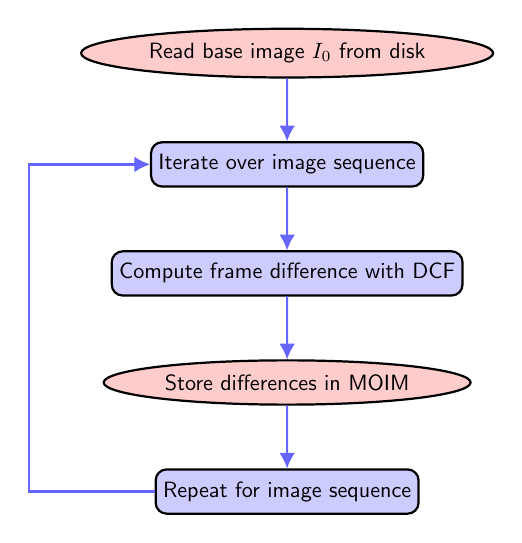
\begin{tikzpicture}[
        scale=0.80, every node/.style={scale=1, transform shape},
        font=\sffamily,
        >={Latex[width=2mm,length=2mm]},
        base/.style={draw, thick, align=center, minimum height=2em, minimum width=3em, fill=blue!20},
        process/.style={base, rectangle, rounded corners},
        data/.style={base, ellipse, fill=red!20},
        arrow/.style={->, thick, color=blue!60},
    ]

    % Nodes
    \node[data] (read) {Read base image $I_{0}$ from disk};
    \node[process, below=of read] (iterate) {Iterate over image sequence};
    \node[process, below=of iterate] (compute) {Compute frame difference with DCF};
    \node[data, below=of compute] (store) {Store differences in MOIM};
    \node[process, below=of store] (repeat) {Repeat for image sequence};

    % Arrows
    \draw[arrow] (read) -- (iterate);
    \draw[arrow] (iterate) -- (compute);
    \draw[arrow] (compute) -- (store);
    \draw[arrow] (store) -- (repeat);
    \draw[arrow] (repeat.west) -- ++(-2,0) |- (iterate.west);

    \end{tikzpicture}
    \caption{Proposed Workflow for Inter-frame Encoding}
    \label{fig:figure4}
\end{figure}

\section{Implementation}
This section outlines the implementation of the proposed algorithm, focusing on the pseudo-algorithm for the theoretical approach.

\subsection{Pseudo-Algorithm}
The pseudo-algorithm describes the process of compressing and decompressing image frames using inter-frame encoding based on a temporal redundancy, leveraging Huffman coding and DCT techniques to improve singular compression ratios at image level and relying on techniques described DCF and MOIF, which work at storage level. The process is presented in mathematical terms to illustrate the relationship with the theory described in this document.

\begin{enumerate}
    \item \textbf{Initialization:}
    \begin{itemize}
        \item Set the inception frame $I_0$ as the reference frame.
        \item Initialize an empty set $S$ for storing compressed frame differences.
    \end{itemize}

    \item \textbf{Forming $K$ using $DCF$ (Dynamic Cluster Formation):}
    \begin{enumerate}
        \item Continuously form $K$ clusters based on the difference threshold from a set of frames.
        \item Store clusters generated as part of a set $K$.
        \item Set the first frame $K_0$ as the reference frame (also known as the inception frame $I_0$)
        \item Implement $MOIM$ step to minimize redundant processing and memory usage (See \ref{appendix:a}).
    \end{enumerate}

    \item \textbf{For each frame $K_n$ inside $K$:}
    \begin{enumerate}
        \item Compute the difference $\Delta K_{n} = K_{n} - K_{n-1}$.
        \item Apply DCT to $\Delta K_{n}$ to obtain frequency components $F_{n}$.
        \item Encode $F_{n}$ using Huffman coding to produce a compressed representation $C_{n}$.
        \item Add $C_{n}$ to the set $S$.
    \end{enumerate}

    \item \textbf{Decompression:}
    \begin{enumerate}
        \item Apply difference stored after $MOIM$ To obtain the difference between frames.
        \item From frames obtained after $MOIM$, apply Huffman decoding to obtain $F_{n}$.
        \item Apply the inverse DCT to $F_{n}$ to obtain $\Delta K_{n}$.
        \item Reconstruct frame $I_n = \Delta I_{n} + I_{n-1}$.
    \end{enumerate}
\end{enumerate}

This section provides a framework for the practical application of the proposed algorithm, detailing the steps required to read, extract, and apply differences between frames based on metadata, thus illustrating the algorithm's in a real-world scenario.

\subsection{Implementation Details}
Implementing inter-frame encoding requires careful consideration of several factors, including file formats, compression techniques, and computational complexity. Various file formats, such as JSON or binary formats, can be used to store image data and metadata efficiently. Additionally, compression techniques, such as run-length encoding or delta encoding, can further reduce storage requirements. It is essential to balance compression ratios with computational overhead to achieve optimal performance. Implementation details like metadata formats and compression techniques can be tailored to the specific requirements of the application although here we recommend a single JSON file format to store the differences between frames and metadata required for reconstruction.

\section{Case Studies}
Encoding here presented has been widely used in video compression standards such as MPEG and H.264 \cite{wiegand2003overview} in the past, although here presented we recommend the applicatiion of the same technique to a cluster. These standards leverage inter-frame encoding to achieve significant reductions in storage size as a whole while maintaining high-quality images without being affected. Additionally, encoding could have applications in medical imaging, surveillance systems, and remote sensing, where storage efficiency is critical and images contain significant temporal redundancy.

\section{Conclusion}
In conclusion, inter-frame coding offers a powerful solution for compressing similar image sequences efficiently since its first appearance. However, this technique has always been applied to video coding. By exploiting the temporal redundancy between consecutive frames, the proposed algorithm can achieve high compression ratios while maintaining the image quality individually. The dynamic group formation step ensures that similar images are grouped together, which enables efficient inter-frame coding. The memory optimization and inter-frame matching step minimizes redundant processing and memory usage, further improving the efficiency of the compression algorithm. The proposed algorithm has the potential to significantly reduce the storage requirements of fast capture devices, making it a valuable tool for a wide range of applications that rely on the uniformity of similar images presented in a time series.

\bibliographystyle{acm}
\bibliography{references}

\clearpage
\newpage
\appendix
\section{Annex A: Utilizing Huffman Coding in MOIM}
\label{appendix:a}
\subsection{Introduction}
Huffman coding \cite{huffman1952method}, a popular method for lossless data compression, can significantly enhance the MOIM step by reducing the amount of data required to represent frame differences. This section explains the process and provides a practical example of its application.

\subsection{Huffman Coding in MOIM}
The MOIM step, crucial for minimizing redundant data and optimizing memory usage, can benefit from Huffman coding by encoding the frame differences more compactly. Huffman coding achieves this by assigning variable-length codes to input characters, with shorter codes for more frequent characters. 

\subsubsection{Example}
Consider a simplified scenario where we have computed the differences between consecutive frames, resulting in a series of values. Given the frame differences:
\[
\begin{array}{ccccccccc}
4 & 1 & 2 & 4 & 4 & 2 & 3 & 1 & 4 \\
\end{array}
\]

Frequency of each difference value:
\[
\begin{array}{|c|c|}
\hline
\text{Value} & \text{Frequency} \\
\hline
1 & 2 \\
2 & 2 \\
3 & 1 \\
4 & 4 \\
\hline
\end{array}
\]

Applying Huffman coding to these differences:
\[
\begin{array}{|c|c|}
\hline
\text{Value} & \text{Huffman Code} \\
\hline
4 & 0 \\
1 & 10 \\
2 & 110 \\
3 & 111 \\
\hline
\end{array}
\]

Thus, the encoded sequence using Huffman codes would be:
\[
\begin{array}{ccccccccc}
0 & 10 & 110 & 0 & 0 & 110 & 111 & 10 & 0 \\
\end{array}
\]

This encoded sequence is significantly shorter than the original representation, demonstrating how Huffman coding can compress data efficiently.

\subsection{Conclusion}
Incorporating Huffman coding into the MOIM step allows for a significant reduction in data size by efficiently encoding frame differences. This process not only saves storage space but also accelerates data processing and retrieval, making it a valuable technique for optimizing inter-frame matching and memory usage in video and image compression systems.

\end{document}
